\documentclass[12pt]{amsart} \usepackage{amscd} \usepackage{epsfig}
\usepackage{color} \usepackage{graphicx} \usepackage{enumerate}
\usepackage{float}
\usepackage{subcaption}

\textheight=9.5in \textwidth = 6.4in \topmargin=-.6in
\oddsidemargin=-.05in \evensidemargin=-.05in \parskip=.02in
\newtheorem*{theorem}{Theorem} \newtheorem{lemma}{Lemma}
\newtheorem{conjecture}{Conjecture}
\newtheorem{proposition}{Proposition}
\newtheorem{definition}{Definition}
\newtheorem{statement}{Statement}
\newtheorem{example}{Example}

\begin{document}
All data from 2016.
\begin{itemize}
\item October min,max data $80,88$ yields a range value of 8.
\item November min,max data is $81,90$ yielding a range value of 9.
\item December min,max data is $78,91$ yielding a range value of 13.
\end{itemize}


\begin{table}[H]
\centering
\caption{El Salvador, San Salvador}
\begin{tabular}{lll}
\hline \hline
October & November & December \\
\hline
88 & 84 & 86 \\
88 & 82 & 86 \\
86 & 84 & 86 \\
86 & 87 & 84 \\
86 & 86 & 78 \\
85 & 85 & 84 \\
84 & 85 & 87 \\
87 & 86 & 88 \\
86 & 88 & 88 \\
87 & 90 & 87 \\
88 & 89 & 88 \\
87 & 89 & 82 \\
86 & 88 & 86 \\
86 & 88 & 86 \\
85 & 87 & 87 \\
87 & 87 & 87 \\
84 & 86 & 87 \\
84 & 86 & 88 \\
80 & 84 & 91 \\
84 & 83 & 87 \\
85 & 83 & 87 \\
86 & 83 & 84 \\
86 & 85 & 86 \\
86 & 87 & 85 \\
85 & 86 & 88 \\
84 & 87 & 88 \\
86 & 84 & 89 \\
86 & 84 & 89 \\
86 & 81 & 89 \\
87 & 86 & 86 \\
87 & NA & 88
\end{tabular}
\end{table}

\section*{Sample Statistics}
The first method we used R to calculate all the sample statistics
after importing all data from a text file.  The text file had
copy-and-paste data from a python file that scraped and extracted the
data from the Wunderground website.

\begin{table}[H]
\centering
\caption{El Salvador, San Salvador}
\begin{tabular}{llll}
\hline \hline 
Statistics & October & November & December \\
n & 31 & 30 & 31 \\
$\sum{x}$ & 2658  & 2570 & 2682 \\
$\sum{x^2}$ & 7,064,964 & 6,604,900 & 7,193,124 \\
$\overline{x}$ & 85.74 & 85.67 & 86.52 \\
$\tilde{x}$ & 86 & 86 & 87 \\
$s$ & 1.59 & 2.19 & 2.39  \\
$s^2$ & 2.53  & 4.49 & 5.41 
\end{tabular}
\end{table}

The R \textit{summary} function outputs all quartiles of a data set.  Results
are below.
\begin{table}[H]
\centering
\caption{El Salvador, San Salvador}
\begin{tabular}{llll}
\hline \hline 
Quartile & October & November & December \\
$Q_{1}$ & 85 & 84 & 86 \\
$Q_{3}$ & 87 & 87 & 88
\end{tabular}
\end{table}

\section*{Visual Information}
The boxplot has the best visual information.  The histogram for each
month are included.
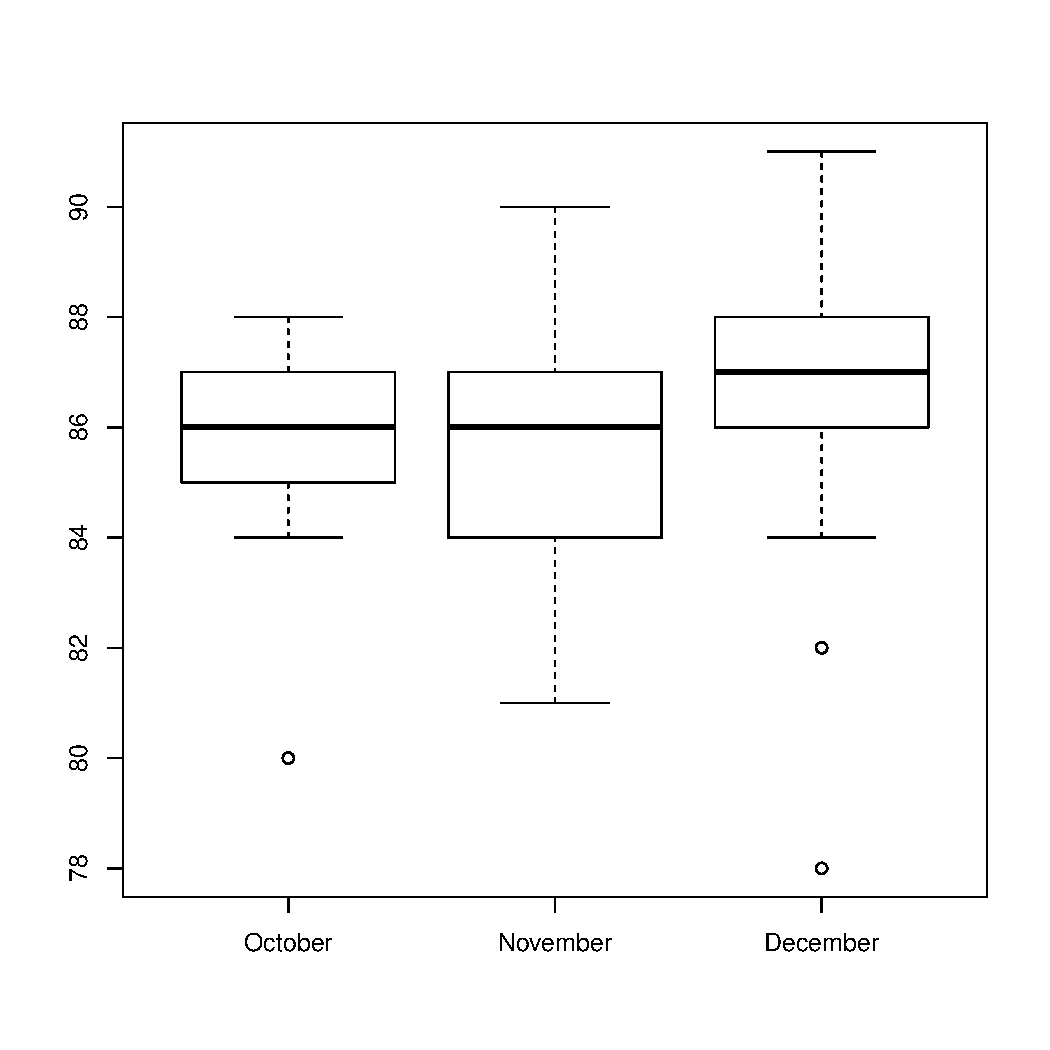
\includegraphics[scale=0.75]{boxplot.pdf}

\begin{figure}
\begin{subfigure}{.33\textwidth}
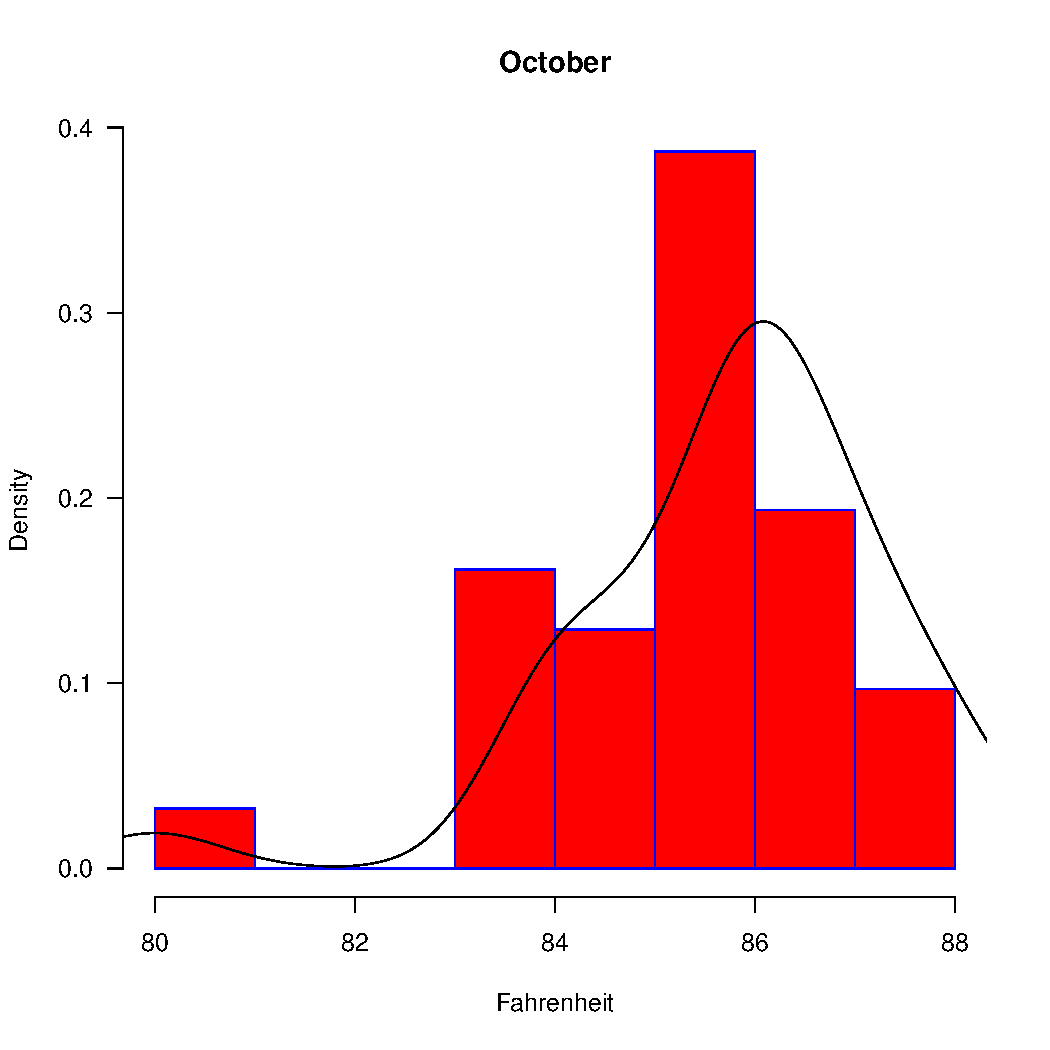
\includegraphics[scale=0.35]{density_october.pdf}
\end{subfigure}

\begin{subfigure}{.33\textwidth}
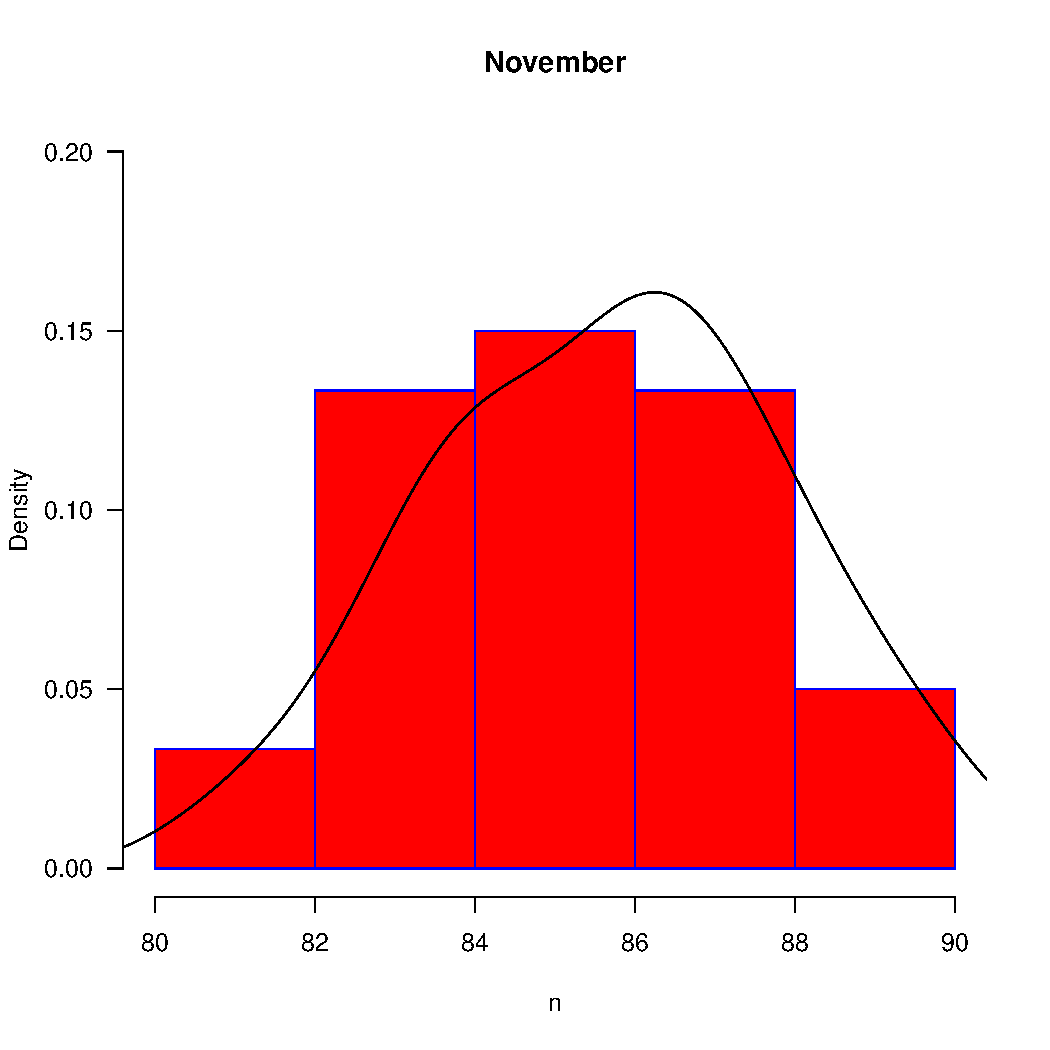
\includegraphics[scale=0.35]{density_november.pdf}
\end{subfigure}

\begin{subfigure}{.33\textwidth}
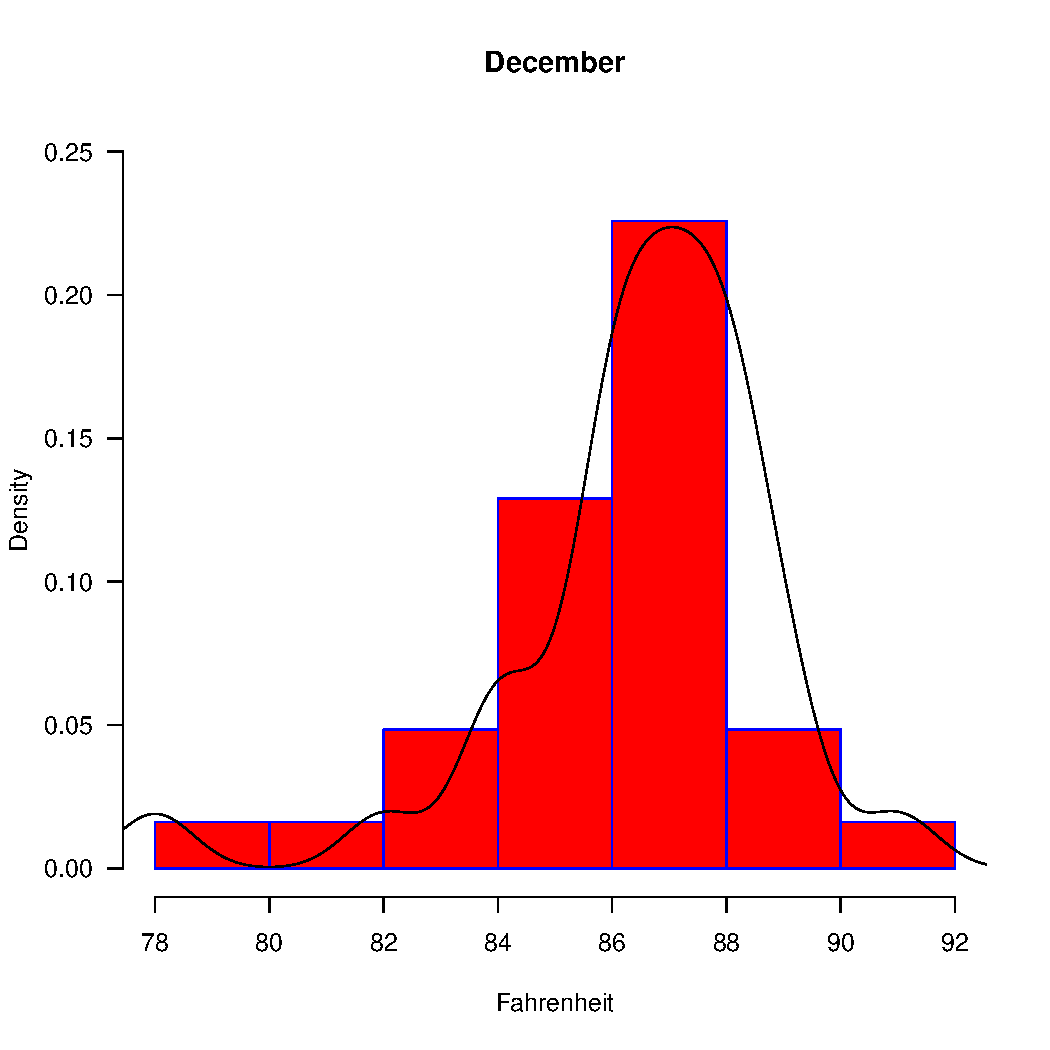
\includegraphics[scale=0.35]{density_december.pdf}
\end{subfigure}
\end{figure}

\end{document}